\documentclass[aspectratio=169,10pt]{beamer}
\usepackage[T1]{fontenc}\usepackage{lmodern}\usepackage{booktabs}\usepackage{tikz}\usepackage{pgfplots}\usepackage{graphicx}
\usetikzlibrary{arrows.meta,positioning}\pgfplotsset{compat=1.17}
\definecolor{navy}{HTML}{173A5E}\definecolor{panel}{HTML}{2D6795}\definecolor{yellow}{HTML}{F4C542}
\definecolor{cyan}{HTML}{70B7DE}\definecolor{green}{HTML}{58B89A}\definecolor{red}{HTML}{E06A70}\definecolor{soft}{HTML}{D8E7F2}
\setbeamercolor{normal text}{fg=white,bg=navy}\setbeamercolor{frametitle}{fg=white,bg=navy}\setbeamercolor{structure}{fg=yellow}
\setbeamercolor{alerted text}{fg=yellow}\setbeamertemplate{navigation symbols}{}
\setbeamertemplate{frametitle}{\vspace{.35em}\hspace{.35em}\insertframetitle\vspace{.25em}}
\setbeamertemplate{footline}{\hfill\color{soft}\scriptsize\insertframenumber\hspace{1em}\vspace{.5em}}
\setbeamercolor{block title}{fg=navy,bg=yellow}\setbeamercolor{block body}{fg=white,bg=panel!55!navy}
\newcommand{\yes}[1]{\textcolor{green}{#1}}\newcommand{\no}[1]{\textcolor{red}{#1}}\newcommand{\key}[1]{\textcolor{yellow}{#1}}
\newcommand{\citecode}[1]{\vfill{\color{soft}\tiny Evidence: \texttt{#1}}}
\begin{document}

\begin{frame}[plain]
\begin{tikzpicture}[remember picture,overlay]\fill[navy] (current page.south west) rectangle (current page.north east);\fill[panel] (current page.south west) rectangle ([xshift=2.1cm]current page.north west);\draw[yellow,line width=2pt] ([xshift=2.1cm]current page.south west)--([xshift=2.1cm]current page.north west);\end{tikzpicture}
\vspace{1.05cm}\hspace{2.3cm}\begin{minipage}{.70\textwidth}
{\LARGE\bfseries Improving semantic movie search}\par\vspace{.45em}
{\large Experiments, implementations and measured outcomes}\par\vspace{1.4em}
{\color{yellow}\bfseries Idea $\rightarrow$ implementation $\rightarrow$ comparison $\rightarrow$ verdict}\par\vspace{1.6em}
{\small Master 2 project \hfill July 2026}\end{minipage}
\end{frame}

\begin{frame}{How every experiment is presented}
Each experiment follows the same three questions:
\begin{enumerate}
\item \key{Setup and idea:} what problem were we trying to solve?
\item \key{Implementation:} what changed in code or prompts? A concrete example and source citation are provided.
\item \key{Comparison and verdict:} did it beat the previous method, and why?
\end{enumerate}
\vfill
\begin{block}{Quality measures}
Recall = share of correct movies recovered. Precision = share of returned movies that are correct. F1 = balance between precision and recall.
\end{block}
\end{frame}

\begin{frame}{Starting point: two main methods}
\begin{columns}[T]\column{.47\textwidth}\textbf{SUQL Stage 2}
\begin{itemize}\item Cheap model scores each review.\item Strong model checks uncertain cases.\item Designed to save strong-model calls.\end{itemize}
\column{.47\textwidth}\textbf{V3.2}
\begin{itemize}\item Database rules reduce the candidate set.\item Reviews are classified in batches.\item Usually uses only about four model calls per run.\end{itemize}\end{columns}
\vfill
These are the reference methods against which prompt, context, cascade and synonym changes were tested.
\citecode{project SUQL/Stage\_2/README.md:14--55; project Trummer/heterogen\_v3\_2/}
\end{frame}

\begin{frame}{Experiment 1 --- setup: recover missing final rows}
\textbf{Observation:} the database found candidates, but some Gemma4/SUQL runs returned zero movies.
\begin{center}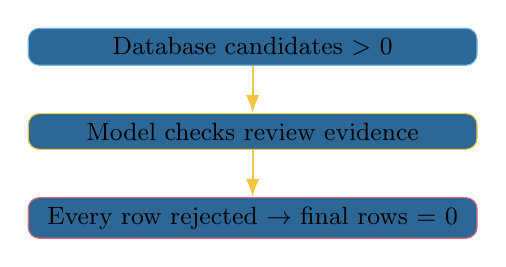
\begin{tikzpicture}[node distance=6mm,every node/.style={font=\small}]
\node[draw=cyan,fill=panel,rounded corners,minimum width=5.7cm] (a) {Database candidates $>$ 0};
\node[draw=yellow,fill=panel,rounded corners,below=of a,minimum width=5.7cm] (b) {Model checks review evidence};
\node[draw=red,fill=panel,rounded corners,below=of b,minimum width=5.7cm] (c) {Every row rejected $\rightarrow$ final rows = 0};
\draw[-{Latex},yellow,thick] (a)--(b);\draw[-{Latex},yellow,thick] (b)--(c);
\end{tikzpicture}\end{center}
\key{Idea:} uncertainty or a scoring failure should trigger a second check, not automatic deletion.
\citecode{test\_project/project SUQL/src\_baseline\_stage2/suql\_engine.py:706--717}
\end{frame}

\begin{frame}{Experiment 1 --- implementation: safer confidence handling}
\begin{columns}[T]\column{.47\textwidth}\textbf{Before}
\begin{block}{Prompt}\ttfamily\scriptsize Classify whether the review answers\\the question with Yes.\\Return exactly one token: 1 or 0.\end{block}
\begin{itemize}\scriptsize\item Expected confidence for both tokens.\item A confident negative could be rejected immediately.\end{itemize}
\column{.49\textwidth}\textbf{After}
\begin{block}{Prompt}\ttfamily\scriptsize Avoid false negatives. If evidence is\\credible, mixed or ambiguous, answer 1.\\Answer 0 only when clearly absent.\end{block}
\begin{itemize}\scriptsize\item Can derive signed confidence from one generated-token probability.\item Missing confidence goes to the stronger model.\item Negative cheap scores are rechecked.\end{itemize}\end{columns}
\citecode{test\_project/project SUQL/Stage\_1/profiler.py:54--60,136--147; Stage\_2/cascade\_filter.py:269--308}
\end{frame}

\begin{frame}{Experiment 1 --- comparison and verdict}
\begin{columns}[T]\column{.47\textwidth}\textbf{Before fix}
\begin{itemize}\item Some 12B$\rightarrow$31B SUQL configurations: recall = \no{0.000}.\item More output tokens still produced zero rows.\end{itemize}
\column{.47\textwidth}\textbf{After recall-first redesign}
\begin{itemize}\item Qwen Stage 2 baseline: recall = \yes{0.692}.\item Final rows were produced again.\item Cost increased to 33.5 calls/run.\end{itemize}\end{columns}
\vfill
\begin{block}{Verdict: succeeded}
The problem was an architecture--model compatibility failure. Models exposed the weakness, but the architectural fix was to recheck uncertainty instead of rejecting it.
\end{block}
\citecode{test\_project/results/baseline\_10q\_10reps/qwen\_comparison/aggregate\_summary.csv}
\end{frame}

\begin{frame}{Experiment 2 --- setup and implementation: extra examples}
\textbf{Idea:} give the model labelled examples of recommendation, chemistry and ending evidence before it judges a new review.
\begin{block}{Example added to the prompt}
\ttfamily\scriptsize Ground-truth examples for this exact task:\\
Example 1 review: [known review]\\
Example 1 label: Yes\\
Apply the same distinction to the new review.
\end{block}
The code selected an example group from predicate words, formatted the reviews and labels, and prepended them to the classifier prompt.
\citecode{test\_project/context\_version/fewshot\_context.py:9--24; project SUQL/Stage\_2/cascade\_filter.py}
\end{frame}

\begin{frame}{Experiment 2 --- comparison and verdict}
\centering
\begin{tabular}{lrrr}\toprule Method & Previous recall & With examples & Change\\\midrule
Stage 2 & 0.556 & 0.194 & \no{$-$0.361}\\
V3.2 & 0.611 & 0.556 & \no{$-$0.056}\\\bottomrule\end{tabular}
\vfill
\begin{block}{Verdict: failed}
The extra reviews made prompts longer and introduced distracting evidence. The model became slower and more conservative instead of transferring the intended distinction.
\end{block}
\citecode{test\_project/context\_version/results/3q\_context\_qwen35\_1rep/comparison\_averages.csv}
\end{frame}

\begin{frame}{Experiment 3 --- setup: expert synonym guidance}
\textbf{Idea:} provide a short list of human-selected ways to express the same concept.
\begin{block}{Example for romantic chemistry}
\ttfamily\scriptsize Semantic family: relationship\_and\_chemistry\_praise.\\
Look for these signals and natural paraphrases:\\
chemistry, convincing couple, believable relationship, romance works.\\
The terms are recall cues, not exact-match requirements.
\end{block}
The guide was attached to the semantic predicate before model classification.
\citecode{test\_project/generalized\_synonym\_version/predicate\_synonyms.py:48--59}
\end{frame}

\begin{frame}{Experiment 3 --- comparison and verdict}
\centering
\begin{tabular}{lrrr}\toprule Method & Previous recall & Expert cues & Change\\\midrule
Stage 2 & 0.556 & 0.583 & \yes{+0.028}\\
V3.2 & 0.611 & 0.667 & \yes{+0.056}\\\bottomrule\end{tabular}
\vfill
\begin{block}{Verdict: small success}
Short, question-specific paraphrases helped the model recognize alternative wording. The gain was modest because broader acceptance also reduced precision.
\end{block}
\citecode{test\_project/synonym\_version/results/3q\_dynamic\_synonyms\_qwen35/comparison\_averages.csv}
\end{frame}

\begin{frame}{Experiment 4 --- setup and implementation: learned cues}
\textbf{Idea:} learn vocabulary automatically instead of writing every synonym by hand.
\begin{columns}[T]\column{.47\textwidth}\textbf{Lexical learner}
\begin{itemize}\item Selects words/phrases correlated with positive examples.\item Risk: frequent artifacts look predictive.\end{itemize}
\column{.47\textwidth}\textbf{Ground-truth concept learner}
\begin{itemize}\item Uses known positive movies to organize cues into semantic topics.\item Aims to learn meanings rather than isolated tokens.\end{itemize}\end{columns}
\vfill
Both produced a JSON guide mapping each question to a semantic family and cue categories.
\citecode{test\_project/learned\_synonym\_version/learn\_synonym\_guide.py; ground\_truth\_synonym\_version/learn\_synonym\_guide.py}
\end{frame}

\begin{frame}{Experiment 4 --- comparison and verdict}
\centering\small
\begin{tabular}{llrr}\toprule Variant & Method & Recall & Change vs baseline\\\midrule
Lexical learning & Stage 2 & 0.361 & \no{$-$0.194}\\
Lexical learning & V3.2 & 0.306 & \no{$-$0.306}\\
GT concepts & Stage 2 & 0.361 & \no{$-$0.194}\\
GT concepts & V3.2 & 0.583 & \no{$-$0.028}\\\bottomrule\end{tabular}
\vfill
\begin{block}{Verdict: lexical failed; concept learning was partial}
Lexical selection learned accidental correlations and dataset artifacts. Semantic supervision repaired much of the V3.2 damage, but did not consistently beat expert cues.
\end{block}
\citecode{test\_project/*synonym\_version/results/3q\_*/comparison\_averages.csv}
\end{frame}

\begin{frame}{Experiment 5 --- setup: learn from a larger 5k sample}
\textbf{Idea:} improve coverage by learning concepts from 5,000 IMDb rows while preventing benchmark leakage.
\begin{itemize}
\item Excluded all 600 benchmark movies.
\item Split remaining movies into training and validation sets by movie.
\item Started from high-precision seed cues.
\item Added phrases only when they improved validation recall above a precision threshold.
\end{itemize}
\vfill
Example: recommendation learning used 688 pseudo-positive movies and selected 9 cues.
\citecode{test\_project/generalized\_synonym\_version/learn\_full\_dataset\_synonyms.py; full5k\_concept\_learning\_report.json}
\end{frame}

\begin{frame}{Experiment 5 --- implementation: what the model actually sees}
\textbf{Learned recommendation cues}
\begin{block}{Guide entry}
\ttfamily\scriptsize paraphrases: must see, worth watching, worth seeing,\\
recommend seeing, recommend watching\\
implicit signals: worth a watch, end i recommend,\\
recommend that you see
\end{block}
\textbf{Prompt prefix sent to the model}
\begin{block}{Rendered guidance}
\ttfamily\scriptsize Learned semantic concept: explicit\_recommendation.\\
Paraphrases: must see, worth watching, ...\\
Implicit signals: worth a watch, ...\\
These are semantic examples, never exact-match rules. Accept unseen wording.
\end{block}
This prefix is concatenated before the review and question in both Stage 2 and V3.2.
\citecode{predicate\_synonyms.py:43--76; project SUQL/Stage\_2/cascade\_filter.py:343--353; heterogen\_v3\_2/trummer\_join/cascade.py:546--574}
\end{frame}

\begin{frame}{Experiment 5 --- comparison and verdict}
\centering\scriptsize
\begin{tabular}{llrrr}\toprule Variant & Method & Precision & Recall & F1\\\midrule
No guide & Stage 2 & .652 & .491 & .520\\
Small guide & Stage 2 & .732 & \yes{.591} & \yes{.610}\\
Full-5k guide & Stage 2 & \yes{.743} & .528 & .576\\\midrule
No guide & V3.2 & .692 & .481 & .546\\
Small guide & V3.2 & \yes{.743} & .556 & .617\\
Full-5k guide & V3.2 & .733 & \yes{.583} & \yes{.636}\\\bottomrule\end{tabular}
\vfill
\begin{block}{Verdict: succeeded for V3.2, partial for Stage 2}
More data improved V3.2 recall and F1. It did not beat the smaller guide for Stage-2 recall: frequent phrases can displace rare, question-specific cues. Matched Q1--Q9 only; Q10 is incomplete.
\end{block}
\citecode{test\_project/results/gemma4\_baseline\_vs\_small\_vs\_full5k\_synonyms/matched\_aggregate.csv}
\end{frame}

\begin{frame}{Experiment 6 --- setup and implementation: three model levels}
\textbf{Idea:} add a middle model to recover hard candidates before final adjudication.
\begin{enumerate}
\item Qwen 4B: fast pass for explicit evidence.
\item Granite 8B: recovery pass over rejected rows; searches for paraphrases and indirect evidence.
\item Qwen 9B: final decision over surviving candidates, or all candidates when recovery is short.
\end{enumerate}
Each model returned structured JSON decisions for every candidate.
\citecode{test\_project/three\_level\_version/three\_level\_pipeline.py:55--104,107--128}
\end{frame}

\begin{frame}{Experiment 6 --- comparison and verdict}
\centering
\begin{tabular}{lrrr}\toprule Method & Two-level recall & Three-level recall & Change\\\midrule
Stage 2 & .556 & .139 & \no{$-$.417}\\
V3.2 & .611 & .083 & \no{$-$.528}\\\bottomrule\end{tabular}
\vfill
\begin{block}{Verdict: failed}
Every additional model boundary created another opportunity to reject a correct movie. Errors accumulated, while runtime rose to roughly 300 seconds.
\end{block}
\citecode{test\_project/three\_level\_version/results/3q\_three\_level\_qwen\_granite\_qwen/comparison\_averages.csv}
\end{frame}

\begin{frame}{Overall conclusions by method}
\small\begin{tabular}{p{3.1cm}p{1.7cm}p{6.1cm}}\toprule Method & Verdict & Simple reason\\\midrule
Recall-first confidence fix & \yes{Success} & Prevented uncertainty from silently deleting candidates.\\
Extra labelled context & \no{Failed} & Added prompt noise and conservative decisions.\\
Expert synonyms & \yes{Small gain} & Short cues matched the questions well.\\
Lexical learning & \no{Failed} & Learned correlations rather than stable meaning.\\
GT concept learning & Partial & Better semantics, but inconsistent generalization.\\
Full-5k learning & Partial / useful & Best V3.2 quality; smaller guide kept better Stage-2 recall.\\
Three-level cascade & \no{Failed} & More rejection points compounded errors.\\
V3.2 & \yes{Best balance} & Strong quality with about four calls per run.\\\bottomrule\end{tabular}
\end{frame}

\begin{frame}{Final recommendation}
\begin{enumerate}
\item Use \key{V3.2 + full-5k guide} for the best current balance of precision, recall, F1 and calls.
\item Use \key{Stage 2 + small guide} when recall is the priority and runtime is less important.
\item Keep the recall-first fallback rule in every method: scoring failure must never equal rejection.
\item Keep prompts short and task-specific; do not add context or model stages without proving a recall gain.
\item Finish Q10 and validate on unseen movies before making a full ten-question generalization claim.
\end{enumerate}
\end{frame}

\end{document}
